\begin{frame}
\frametitle{Average Sim}
The first simulation is an example facility with the following input values:
\begin{itemize}
	\item Temperature -- 900 $^\circ$ C
	\item Pressure -- 500 mTorr
	\item Rotation -- 100 rpm
	\item Current -- 8 A
	\item Time -- 1 hr
\end{itemize}
The simulation is run for 20 time steps with simple source and sink archetypes to facilitate trading.

This scenario was run to verify trading capabilities and general separations.
\end{frame}

\begin{frame}
\frametitle{Average Sim - Results}
\begin{columns}
	\begin{column}{.5\textwidth}
		\begin{figure}
			\centering
			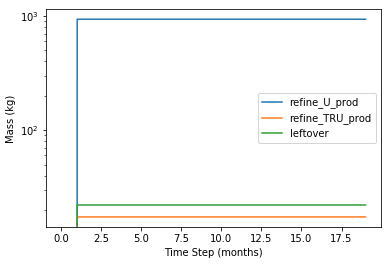
\includegraphics[width=\linewidth]{timeseries-prod}
			\caption{Product time series of a simple simulation.}
			\label{fig:timeseries-prod}
		\end{figure}
	\end{column}
	\begin{column}{.5\textwidth}
		\begin{figure}
			\centering
			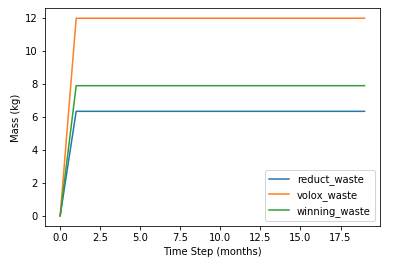
\includegraphics[width=\linewidth]{timeseries-waste}
			\caption{Waste time series of a simple simulation.}
			\label{fig:timeseries-waste}
		\end{figure}
	\end{column}
\end{columns} 
\end{frame}

\begin{frame}
\frametitle{Isotopic Composition of Waste Streams}
  \begin{figure}
  	\centering
  	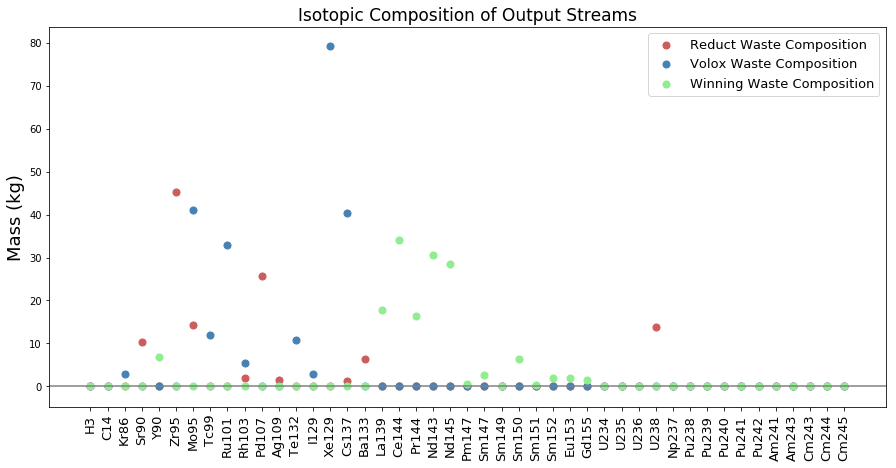
\includegraphics[width=\linewidth]{avg-isotope-comp}
  	\caption{Isotopic Composition of Average Waste Streams}
  	\label{fig:avg-isotope-comp}
  \end{figure}
\end{frame}

\begin{frame}
\frametitle{High Current Simulation}
Secondly, a scenario was run with a current increase from 8 amps to 10 amps to observe
potential diverted material.
\begin{itemize}
	\item Temperature -- 900 $^\circ$ C
	\item Pressure -- 500 mTorr
	\item Rotation -- 100 rpm
	\item Current -- 10 A
	\item Time -- 1 hr
\end{itemize}
The simulation is run for 20 time steps with simple source and sink archetypes to facilitate trading.

We expect only Electroreduction and Electrowinning streams to change.
\end{frame}

\begin{frame}
\frametitle{Current Diversion}
  \begin{figure}
  	\centering
  	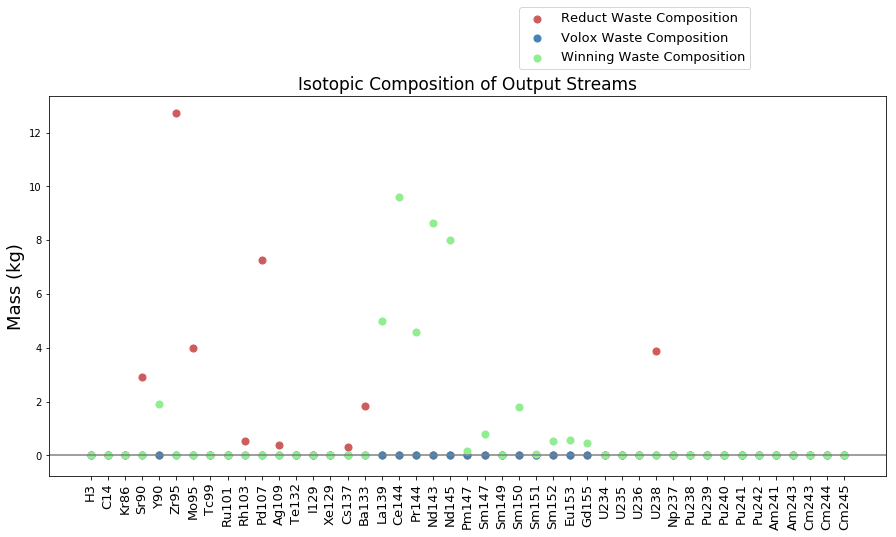
\includegraphics[width=\linewidth]{current-isotope-comp}
  	\caption{Isotopic Composition of Current Diverted Waste Streams}
  	\label{fig:current-isotope-comp}
  \end{figure}
\end{frame}

\begin{frame}
\frametitle{Max Diversion Scenario}
Finally, a simulation was created to observe the maximum possible material discrepancy.
This was done by running two separate simulations, one with each parameter at their maximum
efficiency and the other at their minimums. The difference of these results will show how much of each material can be diverted.
\begin{itemize}
	\item Temperature -- 1000 $^\circ C$ vs. 500 $^\circ C$
	\item Pressure -- 120 mTorr vs. 760 mTorr
	\item Rotation -- 100 rpm vs. 0 rpm
	\item Current -- 10 A vs. 4 A
	\item Time -- 4 hr vs. 1 hr
\end{itemize}
The simulation is run for 20 time steps with simple source and sink archetypes to facilitate trading.

Note: The values shown are cumulative over 20 transactions/months (Pu is of interest)
\end{frame}

\begin{frame}
  \frametitle{Isotopic Range}
  \begin{figure}
  	\centering
  	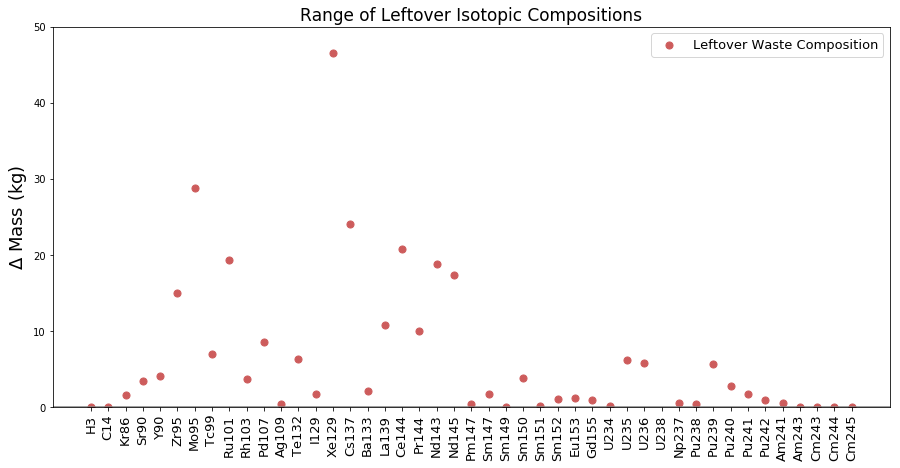
\includegraphics[width=\linewidth]{isotopic-comp-range}
  	\caption{Range of Isotopic Values}
  	\label{fig:isotopic-range}
  \end{figure}
\end{frame}

